% Extraído de Textuais/04-Resultados.tex
% Cores usadas nesta figura (valores CMYK da paleta dvipsnames do xcolor), definidas aqui para não depender de opções externas
\definecolor{BurntOrange}{cmyk}{0,0.51,1,0}
\definecolor{ForestGreen}{cmyk}{0.91,0,0.88,0.12}
\definecolor{BrickRed}{cmyk}{0,0.89,0.94,0.28}
\begin{table}[htbp]
    \centering
    \footnotesize
    \caption{\textit{Features} ordenadas pela taxa média de mudança no período de teste: real e prevista}
    \label{tab:res-ranking}
    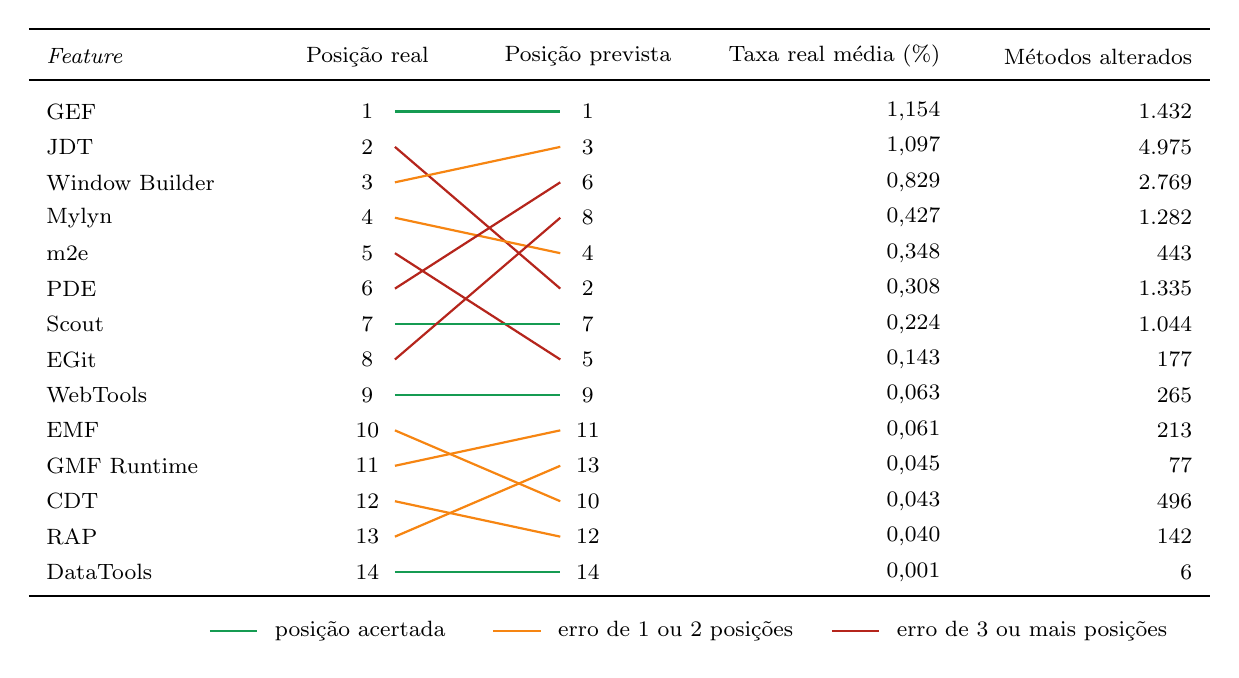
\begin{tikzpicture}[x=1cm, y=1cm, font=\footnotesize, text=black]
        % linha k (k = posição real) fica em y = -0,45k - 0,25
        \def\ylin#1{-0.45*#1-0.25}
        \draw[black, line width=0.8pt] (-0.1,0.35) -- (14.9,0.35);
        \node[anchor=west] at (0,0) {\textit{Feature}};
        \node at (4.2,0) {Posição real};
        \node at (7.0,0) {Posição prevista};
        \node[anchor=east] at (11.6,0) {Taxa real média (\%)};
        \node[anchor=east] at (14.8,0) {Métodos alterados};
        \draw[black, line width=0.5pt] (-0.1,-0.3) -- (14.9,-0.3);
        % feature / posição real / posição prevista / taxa / métodos alterados
        \foreach \f/\r/\p/\t/\m in {GEF/1/1/{1,154}/{1.432}, JDT/2/3/{1,097}/{4.975},
                Window Builder/3/6/{0,829}/{2.769}, Mylyn/4/8/{0,427}/{1.282}, m2e/5/4/{0,348}/443,
                PDE/6/2/{0,308}/{1.335}, Scout/7/7/{0,224}/{1.044}, EGit/8/5/{0,143}/177,
                WebTools/9/9/{0,063}/265, EMF/10/11/{0,061}/213, GMF Runtime/11/13/{0,045}/77,
                CDT/12/10/{0,043}/496, RAP/13/12/{0,040}/142, DataTools/14/14/{0,001}/6} {
            \node[anchor=west] at (0,{\ylin{\r}}) {\f};
            \node at (4.2,{\ylin{\r}}) {\r};
            \node at (7.0,{\ylin{\r}}) {\p};
            \node[anchor=east] at (11.6,{\ylin{\r}}) {\t};
            \node[anchor=east] at (14.8,{\ylin{\r}}) {\m};
        }
        % ligações: posição real k -> linha da feature que o modelo colocou na posição k
        % cor pelo erro |k - j| em posições: 0 = acerto, 1 a 2 = erro pequeno, 3 ou mais = erro grande
        \foreach \k/\j in {1/1, 2/6, 3/2, 4/5, 5/8, 6/3, 7/7, 8/4, 9/9, 10/12, 11/10, 12/13, 13/11, 14/14} {
            \pgfmathtruncatemacro{\erro}{abs(\k-\j)}
            \ifnum\erro=0 \def\cor{ForestGreen}\else\ifnum\erro<3 \def\cor{BurntOrange}\else \def\cor{BrickRed}\fi\fi
            \draw[\cor, thick] (4.55,{\ylin{\k}}) -- (6.65,{\ylin{\j}});
        }
        \draw[black, line width=0.8pt] (-0.1,{\ylin{14}-0.3}) -- (14.9,{\ylin{14}-0.3});
        % legenda das ligações
        \begin{scope}[shift={(2.2,{\ylin{14}-0.75})}, text=black]
            \draw[ForestGreen, thick] (0,0) -- (0.6,0);
            \node[anchor=west] at (0.7,0) {posição acertada};
            \draw[BurntOrange, thick] (3.6,0) -- (4.2,0);
            \node[anchor=west] at (4.3,0) {erro de 1 ou 2 posições};
            \draw[BrickRed, thick] (7.9,0) -- (8.5,0);
            \node[anchor=west] at (8.6,0) {erro de 3 ou mais posições};
        \end{scope}
    \end{tikzpicture}
    \fonte{Elaborado pelo autor (2026)}
\end{table}%
